\chapter{Nonequispaced Discrete Spherical Fourier Transform}
\label{DSFT}
Let in this chapter $M \in \NZ$ be a fixed \emph{bandwidth}, $N := 2^{\ceil{\log_2 M}}$ be the 
next greater power of two with respect to $M$, $D \in \N$ and $\mathcal{X} := \paren{\vtheta_d,\vphi_d}_{d=0,\ldots,D-1}$ 
an ordered set of nodes on $\twosphere$ called the \emph{sampling set}.

The concern of the \emph{discrete spherical Fourier transform (DSFT)} 
is to evaluate a function $f: \twosphere \rightarrow \C$, $f \in \fun{\Pol_{M}}{\twosphere}$ given its Fourier expansion
\begin{equation}
  \label{NFSFT:FourierExpansion} 
  f = \sum_{\paren{k,n} \in\mathcal{I}^M} \fun{a_k^n}{f} Y_{k}^n = \sum_{k=0}^M \sum_{n=k}^k \fun{a_k^n}{f} Y_{k}^n = \sum_{n=-M}^M \sum_{k=\abs{n}}^M \fun{a_k^n}{f} Y_{k}^n,
\end{equation}  
on the sampling set $\mathcal{X}$, where $$\mathcal{I}^M := \pset{\paren{k,n}}{|}{k=0,\ldots,M;n=-k,\ldots,k}.$$
We call $M$ the \emph{bandwidth} of $f$ and $a_{k}^n = \fun{a_k^n}{f}$ are the \emph{spherical Fourier coefficients} of $f$ with respect to the 
orthonormal basis of spherical harmonics $\set{Y_{k}^n}_{\paren{k,n} \in\mathcal{I}^M}$ of $\fun{\Pol_{M}}{\twosphere}$. The Fourier coeffcients $a_{k}^n$ may be ordered 
in different ways. We refer to the \emph{degree-mayor order} when the Fourier coefficents are sorted first by degree $k$ and then by order $n$ in ascending order, hence
$$ a_{0}^0, a_{1}^{-1}, a_{1}^{0}, a_{1}^{1}, a_{2}^{-2}, \ldots, a_{M}^{M-1}, a_{M}^{M}.$$ 
Analogously, the \emph{order-mayor order} corresponds to reversed precedence, i.e.
$$ a_{M}^{-M}, a_{M-1}^{-(M-1)}, a_{M}^{-(M-1)}, a_{M-2}^{-(M-2)}, \ldots, a_{M-1}^{M-1}, a_{M}^{M-1}, a_{M}^{M}.$$ 

From a linear algebra point of view, evaluating $f$ on $\mathcal{X}$ corresponds to a matrix-vector product
$$ \V{f}_{\mathcal{X}} = \V{Y}_{M,\mathcal{X}} \; \V{a}_{M}$$
with
\begin{equation}
  \nonumber
  \begin{split}
    \V{f}_{\mathcal{X}} & := \paren{f_d}_{d=0}^{D-1} \in \C^{D},\ f_{d} := \fun{f}{\vtheta_{d},\vphi_{d}},\\
    \V{Y}_{M,\mathcal{X}} & := \paren{\fun{Y_k^n}{\vtheta_d,\vphi_d}}_{d=0,\ldots,D-1, \paren{k,n} \in \mathcal{I}^M} \in \C^{D \times \paren{M+1}^2},\\
    \V{a}_{M} & := \paren{a_k^n}_{\paren{k,n} \in \mathcal{I}^M} \in \C^{\paren{M+1}^2}.
  \end{split}
\end{equation}
If not specified otherwise, $\V{a}_{M}$ contains the Fourier coeffcients $a_{k}^n$ in degree-mayor order and the columns of $\V{Y}_{M,\mathcal{X}}$ 
are ordered correspondingly. We drop the indices $\mathcal{X}$ and $M$ if they could be chosen arbitrarily or are obvious from the 
context and write $\V{f} = \V{Y} \; \V{a}$.

A first naive approach to evaluating $f$ on $\mathcal{X}$ according to \eqref{NFSFT:FourierExpansion} would be to compute first all $D\:(M+1)^2$
entries of $\V{Y}$ and then perform the matrix-vector multiplication $\V{Y} \: \V{a}$ in the standard way. This would lead to an $\bigo{M^3 \: D}$
algorithm, since the evaluation of a function $Y_{k}^n$ at a single node already needs $\bigo{M}$ \emph{floating-point operations (flops)}.
But one can do better. Algorithm \ref{NFSFT:directDSFT} referred to as \emph{direct DSFT} computes 
for every $\paren{\vtheta_{d},\vphi_{d}} \in \mathcal{X}$ first the sums 
\begin{equation}
  \label{NFSFT:directDSFT:firstSum}
  \fun{b^{n}}{d} = \sum_{k=\abs{n}}^M a_{k}^n \fun{P_{k}^{\abs{n}}}{\cos\vtheta_{d}}. 
\end{equation}
Here one can employ the \emph{Clenshaw algorithm} (see for example \cite{prtevefl}) using the three-term recurrence 
from \eqref{Basics:AssociatedLegendreDefinition} or \eqref{Basics:AssociatedLegendreDefinition} for the associated 
Legendre functions. We finally compute
$$
  \fun{f}{\vtheta_{d},\vphi_{d}} = \sum_{n=-M}^M \fun{b^{n}}{d} \e^{\im n \vphi_{d}}
$$
directly.
\begin{algorithm}[tb]
  \caption{Direct NDSFT}
  \label{NFSFT:directDSFT}    
  \begin{algorithmic}
    \STATE  Input: $M \in \NZ$, $D \in \N$, $\V{a}_{M}$, $\mathcal{X}$ %$\paren{a_{k}^n}_{\paren{k,n} \in I^M}$
    \STATE
    \FOR {$d=0,\ldots,D-1$} 
      \STATE $f_{d} := 0$
      \FOR {$n=-M,\ldots,M$} 
        \STATE Compute $\fun{b^{n}}{d}$ by the Clenshaw algorithm,
        \STATE $f_{d} := f_{d} + \fun{b^n}{d} * \e^{\im n \vphi_{d}}$
      \ENDFOR
    \ENDFOR
    \STATE
    \STATE Output: $\paren{f_{d}}_{d=0,\dots,D-1}$
\end{algorithmic}
\end{algorithm}
Each application of the Clenshaw algorithm in \eqref{NFSFT:directDSFT:firstSum} needs $\bigo{M}$ 
flops summing up to $\bigo{M^2}$ flops for the complete inner loop. In 
total we have an $\bigo{M^2\:D}$ algorithm for the evaluation of $f$ on $\mathcal{X}$ and gained an order of complexity with respect to $M$. 
For special sampling sets one can do better by exploiting the grid 
structure and employing FFT techniques (Hier sollten dann noch reichlich Referenzen hin). Our aim, however, 
is not to develop algorithms designed for special grids but to describe a general approach to fast 
spherical Fourier transforms for arbitrary sampling sets.

\section{Computing Fourier Coeffcients from Function Samples}
A \emph{discrete Fourier transform} on the torus $\mathbb{T} = \R/\Z$ of length $M \in \N$ can be represented 
as a maxtrix-vector product
$$
  \V{f} = \V{F}_{M} \: \V{\hat{f}}, \quad \V{F}_{M} \in \C^{M \times M},\ \V{\hat{f}},\:\V{f} \in \C^{M}
$$
as well. The Fourier matrix $\V{F}$ is unitary yielding the inversion formula
\begin{equation}
  \label{NFSFT:DFTInversion}
  \V{\hat{f}} = \V{F}^{\h} \: \V{f}
\end{equation}
immediately. The DFT evaluates a trigonometric polynomial 
$$
  f := \sum_{k=0}^{M-1} \fun{\hat{f}}{k} \e^{2 \pi \im k x}
$$
at equidistant nodes $\paren{x_{d}}_{d=0}^{M-1}$ with $x_{d} := \frac{d}{M} \in \mathbb{T}$. 
For an arbitrary sampling set $\mathcal{Z} \subset \mathbb{T}$ the associated Fourier matrix $\V{F}_{\mathcal{Z}}$ is in general no longer unitary. 
Depending on the number of Fourier coefficients $\fun{\hat{f}}{k}$ and the number of nodes, the matrix
$\V{F}$ moreover is no longer square.

Having defined the DSFT as the evaluation of a bandlimited function $f$ on a sampling set $\mathcal{X}$ on $\twosphere$, arises the question 
whether there exist sets $\mathcal{X}$ allowing for an inversion formula similar to \eqref{NFSFT:DFTInversion}.
The answer is affirmative but in general the number of nodes needed exceeds the number of Fourier coefficients to be computed, 
i.e. $\V{Y}_{M,\mathcal{X}}$ is not square.

We want to recover the Fourier coefficients $\V{a}_{M}$ from samples $\V{f}_{\mathcal{X}}$ at certain nodes $\mathcal{X}$. The 
Fourier coefficients $a_{k}^n$ are given by the scalar products
$$
  a_{k}^n = \scalarproduct{f}{Y_{k}^n}_{\twosphere} = \int_{0}^{2\pi} \int_{0}^{\pi} \fun{f}{\vtheta,\vphi} \overline{\fun{Y_{k}^n}{\vtheta,\vphi}} \sin \vtheta \; \dx \vtheta \; \dx \vphi \quad \paren{\paren{k,n} \in \mathcal{I}^M}.
$$
By seperating the integrand with respect to the integration variables, we obtain
\begin{eqnarray*}
  a_{k}^n & = & \int_{0}^{2\pi} \int_{0}^{\pi} \fun{f}{\vtheta,\vphi} \fun{P_{k}^{\abs{n}}}{\cos \vtheta} \e^{-\im n \vphi} \sin \vtheta \; \dx \vtheta \; \dx \vphi\\
          & = & \int_{0}^{\pi} \fun{P_{k}^{\abs{n}}}{\cos \vtheta} \sin \vtheta \; \int_{0}^{2\pi} \fun{f}{\vtheta,\vphi} \e^{-\im n \vphi} \; \dx \vphi \; \dx \vtheta.
\end{eqnarray*}
For the integrals
$$
  \fun{f_{n}}{\vtheta} := \int_{0}^{2\pi} \fun{f}{\vtheta,\vphi} \e^{-\im n \vphi} \; \dx \vphi
$$
we have the quadrature rule
$$ \fun{f_{n}}{\vtheta} = \frac{1}{2(M+1)} \sum_{j=0}^{2(M+1)-1} \fun{f}{\vtheta,\vphi_{j}} \e^{-\im n \vphi_{j}}$$
where
$$ \vphi_{j} := \frac{j\pi}{N} \quad \paren{j=0,\ldots,2(M+1)-1}. $$
This holds due to the Sampling Theorem by taking into account that for fixed $\vtheta$ the function
\begin{eqnarray*}
  \fun{f}{\vtheta,\vphi} & = & \sum_{n=-M}^{M} \left(\sum_{k=\abs{n}}^M a_{k}^n \fun{P_{k}^{\abs{n}}}{\cos \vtheta}\right) \e^{-\im n \vphi}\\
\end{eqnarray*}
is a trigonometric polynomial of degree $M$ in $\vphi$ with Fourier coefficients
$$
  c_{n} := \sum_{k=\abs{n}}^M a_{k}^n \fun{P_{k}^{\abs{n}}}{\cos \vtheta}.
$$
It remains to compute
$$
  a_{k}^n = \int_{0}^{\pi} \fun{P_{k}^{\abs{n}}}{\cos \vtheta} \fun{f_{n}}{\theta} \sin \vtheta \; \dx \vtheta = 
  \int_{-1}^1 \fun{P_{k}^{\abs{n}}}{x} \fun{f_{n}}{\arccos x} \; \dx x.
$$
By verifying that $\fun{P_{k}^{\abs{n}}}{x} \fun{f_{n}}{\arccos x}$ is an algebraic polynomial of degree at most $2M+1$, 
we can use various types of quadrature rules. We first mention the \emph{Gauss-Legendre} quadrature rule
$$
  \int_{0}^{\pi} \fun{P_{k}^{\abs{n}}}{\cos \vtheta} \fun{f_{n}}{\theta} \sin \vtheta \; \dx \vtheta = \sum_{l=0}^{M} w_{l}^{\gl} \fun{P_{k}^{\abs{n}}}{\cos \vtheta_{l}^{\gl}} \fun{f_{n}}{\theta_{l}} 
$$
with nodes $\paren{\vtheta_{l}^{\gl}}_{l=0}^M$ and weights $\paren{w_{l}^{\gl}}_{l=0}^M$ as described for example in \cite{boehme02}. 
We notice that the $M+1$ nodes $\vtheta_{l}^{\gl}$ can be computed as the eigenvalues of the \emph{Jacobi matrix} for the orthogonal 
Legendre polynomial. The weights $w_{l}$ are obtained from the corresponding eigenvectors.

A second idea is to employ a Clenshaw-Curtis quadrature rule
$$
  \int_{0}^{\pi} \fun{P_{k}^{\abs{n}}}{\cos \vtheta} \fun{f_{n}}{\theta} \sin \vtheta \; \dx \vtheta = \sum_{l=0}^{2M} \varepsilon_{l}^{2M} w_{l}^{\cc} \fun{P_{k}^{\abs{n}}}{\cos \vtheta_{l}^{\cc}} \fun{f_{n}}{\theta_{l}}
$$
where $\varepsilon_{0}^{M} := \epsilon_{M}^M := \frac{1}{2}$, $\epsilon_{l}^M := 1$, $l=1,\dots,M-1$, and $\vtheta_{l}^{\cc} = \frac{l\pi}{2M}$ are the \emph{Chebyshev nodes}.
This quadrature rule uses almost twice as many points as the Gauss-Legendre quadrature rule but allows for an easy and fast online computation of the nodes $\vtheta_{l}^{\cc}$
and weights $w_{l}^{\gl}$. The weights are given by
$$ w_{l}^{\gl} = \frac{1}{2M} \sum_{j=0}^{M} \varepsilon_{j}^{M} \frac{-2}{4j^2-1} \cos\frac{lj\pi}{M}.$$
This finally yields for the Fourier coeffcients $a_{k}^n$ the quadrature rules 
\begin{equation}
  \label{NFSFT:iDSFTGL}
  a_{k}^n = \frac{1}{2(M+1)} \sum_{j=0}^{2(M+1)-1} \sum_{l=0}^{M} w_{l}^{\gl} \fun{f}{\vtheta_{l}^{\gl},\vphi_{j}} \overline{\fun{Y_{k}^n}{\vtheta_{l}^{\gl},\vphi_{j}}}
  %a_{k}^n = \frac{1}{2(M+1)} \sum_{j=0}^{2(M+1)-1} \sum_{l=0}^{M} w_{l}^{\gl} \fun{f}{\vtheta_{l}^{\gl},\vphi_{j}} \fun{P_{k}^{\abs{n}}}{\cos \vtheta_{l}^{\gl}} \e^{-\im n \vphi_{j}}
\end{equation}
and
\begin{equation}
  \label{NFSFT:iDSFTCC}
  a_{k}^n = \frac{1}{2(M+1)} \sum_{j=0}^{2(M+1)-1} \sum_{l=0}^{2M} \varepsilon_{l}^{2M} w_{l}^{\cc} \fun{f}{\vtheta_{l}^{\cc},\vphi_{j}} 
  \overline{\fun{Y_{k}^n}{\vtheta_{l}^{\cc},\vphi_{j}}},
\end{equation}
respectively. Associated with this quadrature formulae we define the sampling sets
\begin{eqnarray*}
  \mathcal{X}_{\gl}^M & := & \paren{\vtheta_{l}^{\gl},\vphi_{j}}_{j=0,\dots,2(M+1)-1;l=0,\dots,M},\\
  \mathcal{X}_{\cc}^M & := & \paren{\vtheta_{l}^{\cc},\vphi_{j}}_{j=0,\dots,2(M+1)-1;l=0,\dots,2M}
\end{eqnarray*}
and refer to $\mathcal{X}_{\gl}^M$ as the \emph{Gauss-legendre sampling set of degree M} and to $\mathcal{X}_{\cc}^M$ as the 
\emph{Clenshaw-Curtis sampling set of degree M}. These two types of sampling sets are illustrated in Figure \ref{quadrature}.
\begin{figure}[tb]
  \centering
  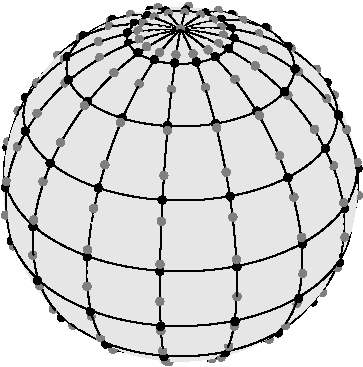
\includegraphics[height=12cm,width=12cm]{images/quadrature}
  \caption{The sample sets $\mathcal{X}_{\gl}^{7}$ (red dots) and $\mathcal{X}_{\cc}^{7}$ (green dots)}
  \label{quadrature}
\end{figure}
We now immediately obtain the corresponding inversion formulae
\begin{align}
  \label{NFSFT:InversionFormulaGL}
  \V{a}_{M} & = \V{Y}_{M,\mathcal{X}_{\gl}}^{\h} \: \V{W}_{\gl} \: \V{f}_{\mathcal{X}_{\gl}}, & \V{W}_{\gl} & := \V{I}_{2M+2} \otimes \diag\paren{w_{l}^{\gl}}_{l=0}^M,\\
  \label{NFSFT:InversionFormulaCC}
  \V{a}_{M} & = \V{Y}_{M,\mathcal{X}_{\cc}}^{\h} \: \V{W}_{\cc} \: \V{f}_{\mathcal{X}_{\cc}}, & \quad \V{W}_{\cc} & := \V{I}_{2M+2} \otimes \diag\paren{\varepsilon_{l}^{2M}w_{l}^{\cc}}_{l=0}^M.
\end{align}  
An algorithm for the multiplication with the adjoint matrix $\V{Y}^{\h}$ is the key for an implementation according to \eqref{NFSFT:InversionFormulaGL} and \eqref{NFSFT:InversionFormulaCC}. Evaluating the matrix-vector product in the standard way, i.e. row-wise, a first approach would be to compute the Fourier coefficients $a_{k}^n$ by \eqref{NFSFT:iDSFTGL} or \eqref{NFSFT:iDSFTCC} for all $\paren{k,n} \in \mathcal{I}^M$ employing the Clenshaw algorithm for the evaluation of the functions $Y_{k}^n$. But this would again lead to an $\bigo{M^3 \: D}$ algorithm. This is due to the fact, that the Clenshaw algorithm would now be applied to each function $Y_{k}^n$ seperately instead of evaluating a linear combination for fixed $n$ and $k = \abs{n},\dots,M$. If we recall that we would end up with a $\bigo{M^3 \: D}$ algorithm for the $DSFT$, too, if we evaluated the matrix $\V{Y}$ componentwise and then performed the matrix-vector multiplication as usual, Algorithm \ref{NFSFT:directDSFT} implies a factorization of $\V{Y}$ into a product of sparse matrices therefore allowing us to save one order of $M$ in computing the matrix-vector product. Furthermore, by taking the adjoint factorization, we immediately obtain a corresponding factorization of $\V{Y}^{\h}$. This allows for the derivation of an algorithm of exactly the same asymptotic complexity for computing the adjoint product.

\section{A Factorization of the Fourier Matrix}

In order to abtain an $\bigo{M^2 \: D}$ algorithm for the adjoint product, we first derive the factorization of $\V{Y}$ according to Algorithm \ref{NFSFT:directDSFT}. The matrix $\V{Y}$ can be written as
$$
  \V{Y} = 
    \left(\begin{array}{c}
      \V{E}_{0}\\
      \V{E}_{1}\\
      \vdots\\
      \V{E}_{D}
    \end{array}\right), \quad \V{E}_{d} \in \C^{1 \times (M+1)^2} \quad \paren{d=0,\ldots,D-1}.
$$
Each matrix $\V{E}_{d}$ evaluates $f$ at $\paren{\vtheta_{d},\vphi_{d}}$ according to 
$$
  \fun{f}{\vtheta_{d},\vphi_{d}} = \sum_{n=-M}^M \sum_{k=\abs{n}}^M a_k^n \fun{Y_{k}^n}{\vtheta_{d},\vphi_{d}}.
$$
So let $d$ be fixed. We begin by evaluating the sums
$$
  \fun{b^{n}}{d} = \sum_{k=\abs{n}}^M a_{k}^n \fun{P_{k}^{\abs{n}}}{\cos\vtheta_{d}} \quad \paren{n=-M,\ldots,M}. 
$$
which corresponds to computing
$$
  \left(\begin{array}{c}
    \fun{b^{-M}}{d}\\
    \fun{b^{-M+1}}{d}\\
    \vdots\\
    \fun{b^{M}}{d}
  \end{array}\right)
  =
  \left(\begin{array}{cccc}
    \fun{\V{C}^{-M}}{d} &                       &        &                    \\
                        & \fun{\V{C}^{-M+1}}{d} &        &                    \\
                        &                       & \ddots &                    \\
                        &                       &        & \fun{\V{C}^{M}}{d} 
  \end{array}\right)
  \:
  \V{a}
$$
where each matrix $\fun{\V{C}^{n}}{d} \in \R^{1 \times (M-n+1)}$ for $n = -M,\ldots,M$ realizes the Clenshaw algorithm acting on the subvector
$$
  \left(\begin{array}{c}
    a_{\abs{n}}^n\\
    a_{\abs{n}+1}^n\\
    \vdots\\
    a_{M}^n\\
  \end{array}\right)  
$$
of $\V{a}$. The matrices $\fun{\V{C}^{n}}{d}$ can be further decomposed corresponding to the number of steps in the Clenshaw algorithm by
\begin{eqnarray*}
  & \fun{\V{C}^{n}}{d} := \prod_{k=\abs{n}+1}^M \fun{\V{C}_{k}^{n}}{d}, \quad \fun{\V{C}_{k}^{n}}{d} :=   
    \encl{[}{\V{I}_{k-\abs{n}}, \fun{\V{\tilde{e}}_{k-\abs{n}}}{d}}{]},\\
  & \quad \fun{\V{\tilde{e}}_{l}}{d} := \paren{0,0,\ldots,\gamma_{k}^n,\alpha_{k}^n \vtheta_{d} + \beta_{k}^n}^{\transp} \in \R^{l}.
\end{eqnarray*}
Finally, we compute the sum
$$
  \fun{f}{\vtheta_{d},\vphi_{d}} = \sum_{n=-M}^M \fun{b^{n}}{d} \e^{\im n \vphi_{d}}
$$
by the scalar product
$$
  f_{d} 
  = 
%  \V{E}_{d}
%  \:
%  \V{a}
%  =
  \paren{\e^{\im (-M) \vphi_{d}},\e^{\im (-M+1) \vphi_{d}},\ldots,\e^{\im M \vphi_{d}}}
  \:   
  \left(\begin{array}{c}
    b^{-M}_{d}\\
    b^{-M+1}_{d}\\
    \vdots\\
    b^{M}_{d}
  \end{array}\right).
$$
This gives us the representation
$$
  \V{E}_{d} = \paren{\e^{\im (-M) \vphi_{d}},\e^{\im (-M+1) \vphi_{d}},\ldots,\e^{\im M \vphi_{d}}} \:  
  \left(\begin{array}{cccc}
    \fun{\V{C}^{-M}}{d} &                       &        &                    \\
                        & \fun{\V{C}^{-M+1}}{d} &        &                    \\
                        &                       & \ddots &                    \\
                        &                       &        & \fun{\V{C}^{M}}{d} 
  \end{array}\right).
$$

\section{Adjoint DSFT}

Now we can simply take the factorized decomposition to obtain the sought algorithm. We have to evaluate
$$
  \V{Y}^{\h} \V{f}
  = 
  \paren{
    \V{E}_{0}^{\h},
    \V{E}_{1}^{\h},
    \ldots,
    \V{E}_{D-1}^{\h}
  }
  \:
  \left(\begin{array}{c}
    f_{0}\\
    f_{1}\\
    \vdots\\
    f_{D-1}
  \end{array}\right). 
$$
This decomposition implies the evaluation of the matrix-vector product in a nonstandard way by traversing the 
matrix column-wise instead of row-wise. After each column $\V{E}_{d}$, the result vector is updated with the portion due 
to the product $\fun{\V{E}^{\h}}{d} \: f_{d}$. We obtain
\begin{equation}
  \label{NFSFT:adjointNDSFTFactorization}
  \fun{\V{\tilde{a}}}{d} := \fun{\V{E}^{\h}}{d} \: f_{d}
  =
  \left(\begin{array}{cccc}
    \fun{{\V{C}^{-M}}^{\transp}}{d} &                                   &        &                               \\
                                    & \fun{{\V{C}^{-M+1}}^{\transp}}{d} &        &                               \\
                                    &                                   & \ddots &                               \\
                                    &                                   &        & \fun{{\V{C}^{M}}^{\transp}}{d} 
  \end{array}\right)
  \:
  \left(\begin{array}{c}
    \e^{\im M \vphi_{d}}\\
    \e^{\im (M-1) \vphi_{d}}\\
    \vdots\\
    \e^{\im (-M) \vphi_{d}}
  \end{array}\right).
\end{equation}
A multiplication with a transposed matrix ${\V{C}^{n}_{d}}^{\transp}$ realizes a \emph{"transposed" Clenshaw algorithm} summarized in Algorithm \ref{NFSFT:transposedClenshaw}.
\begin{algorithm}[htb]
  \caption{Transposed Clenshaw Algorithm}
  \label{NFSFT:transposedClenshaw}    
  \begin{algorithmic}
    \STATE  Input: $M \in \NZ$, $n \in \NZ$ with $\abs{n} \le M$, $d$, $\tilde{b}^n_{d}$
    \STATE
    \STATE $\tilde{a}_{\abs{n}-1}^n := \tilde{b}^n_{d}$
    \STATE $\tilde{a}_{\abs{n}}^n := \tilde{b}^n_{d}$
    \FOR {$k=nleg+1,\ldots,M$} 
      \STATE $\tilde{a}_{k}^n := \paren{\alpha_{k}^n\vtheta_{d} + \beta_{k}^n}\tilde{a}_{k-1}^n + \gamma_{k}^n \tilde{a}_{k-2}^n$
    \ENDFOR
    \STATE
    \STATE Output: $\paren{\tilde{a}_{k}^n}_{k=\abs{n},\ldots,M}$
\end{algorithmic}
\end{algorithm}
The complete algorithm can be obtained from \eqref{NFSFT:adjointNDSFTFactorization} directly. It is given in Algorithm \ref{NFSFT:adjointDSFT}.
\begin{algorithm}[htb]
  \caption{Adjoint DSFT}
  \label{NFSFT:adjointDSFT}    
  \begin{algorithmic}
    \STATE  Input: $M \in \NZ$, $D \in \N$, $\V{f}_{M}$, $\mathcal{X}$
    \STATE
    \FOR {$n=-M,\ldots,M$} 
      \FOR {$k=\abs{n},\ldots,M$} 
        \STATE $tilde{a}_{k}^n := 0;$
      \ENDFOR
    \ENDFOR
    \FOR {$d=0,\ldots,D-1$} 
      \FOR {$n=-M,\ldots,M$} 
        \STATE $b_{d}^n := f_{d} \e^{\im n \vphi_{d}}$
        \STATE Compute $\paren{\tilde{a}_{k}^n}_{k=\abs{n}}^{M}$ by the transposed Clenshaw algorithm
        \FOR {$k=\abs{n},\ldots,M$} 
          \STATE $\tilde{a}_{k}^n := \tilde{a}_{k}^n + \tilde{a}_{k}^n$
        \ENDFOR
      \ENDFOR
    \ENDFOR
    \STATE
    \STATE Output: $\paren{\tilde{a}_{k}^n}_{\paren{k,n} \in \mathcal{I}^M}$
\end{algorithmic}
\end{algorithm}

\section{Inverse DSFT}

This leads to the \emph{direct} Algorithms \ref{} and \ref{} and we refer to them as the \emph{inverse discrete spherical Fourier transform} of \emph{Gauss-Legendre type (iDSFT-GL)} and \emph{Clenshaw-Curtis type (iDSFT-CC)}, respectively.
\begin{algorithm}[htb]
  \caption{Direct iNDSFT-GL}
  \label{NFSFT:directDSFT}    
  \begin{algorithmic}
    \STATE  Input: $M \in \NZ$, $f_{j}$ for $\paren{\vtheta_{j}^{\gl},\phi_{j}} \in \mathcal{X}_{\gl}^M$
    \STATE
    \FOR {$k=0,\ldots,M$} 
      \FOR {$n=-k,\ldots,k$} 
        \STATE $a_{k}^n := 0$
        \FOR {$n=-M,\ldots,M$} 
          \STATE Compute $b^{n}_{d}$ by the Clenshaw algorithm,
          \STATE $f_{d} := f_{d} + b_{d}^n * \e^{\im n \vphi_{d}}$
        \ENDFOR  
      \ENDFOR
    \ENDFOR
    \STATE
    \STATE Output: $\paren{f_{d}}_{d=0,\dots,D-1}$
\end{algorithmic}
\end{algorithm}


So by evaluating $f$ on the grid $\paren{\vtheta_{l},\vphi_{j}}_{l=0,\ldots,M;j=0,\ldots,2(M+1)-1}$ we are able to recover the Fourier coefficients by \eqref{} which leads to the following algorithm

\begin{algorithm}[ht]
  \caption{Discrete Spherical Fourier Transform (DSFT)}
  \label{NFSFT:DSFT}    
  \begin{algorithmic}
    \STATE  Input: $M \in \NZ$, $\paren{a_{k}^n}_{\paren{k,n} \in I^M}$
    \STATE
    \STATE Compute $\paren{f_{l,j}}_{l=0,\ldots,M;j=0,\ldots,2(M+1)-1}$ with 
      $$f_{l,j} = \fun{f}{\paren{\vtheta_{l},\vphi_{j}}} = \sum_{n=-M}^{M} \sum_{k=\abs{n}}^M a_{k}^n \fun{Y_{k}^n}{\vtheta_{l,\vphi_{j}}}.$$
    \STATE 
    \FOR {$l=0,\ldots , M$} 
      \FOR {$j=0,\ldots , 2(M+1)-1$} 
        \STATE $\tilde{f}_{l,j} := w_{l} f_{l,j}$
      \ENDFOR
    \ENDFOR
    \STATE
    \STATE Compute $\paren{a_{k}^n}_{\paren{k,n} \in I^M}$ with 
      $$a_{k}^n = \frac{1}{2(M+1)} \sum_{j=0}^{2(M+1)-1} \sum_{l=0}^{M} \tilde{f}_{l,j} \fun{Y_{k}^n}{\vtheta_{l,\vphi_{j}}}.$$
    \STATE
    \STATE Output: $\paren{a_{k}^n}_{\paren{k,n} \in I^M}$
\end{algorithmic}
\end{algorithm}

\begin{figure}[tb]
  \centering
  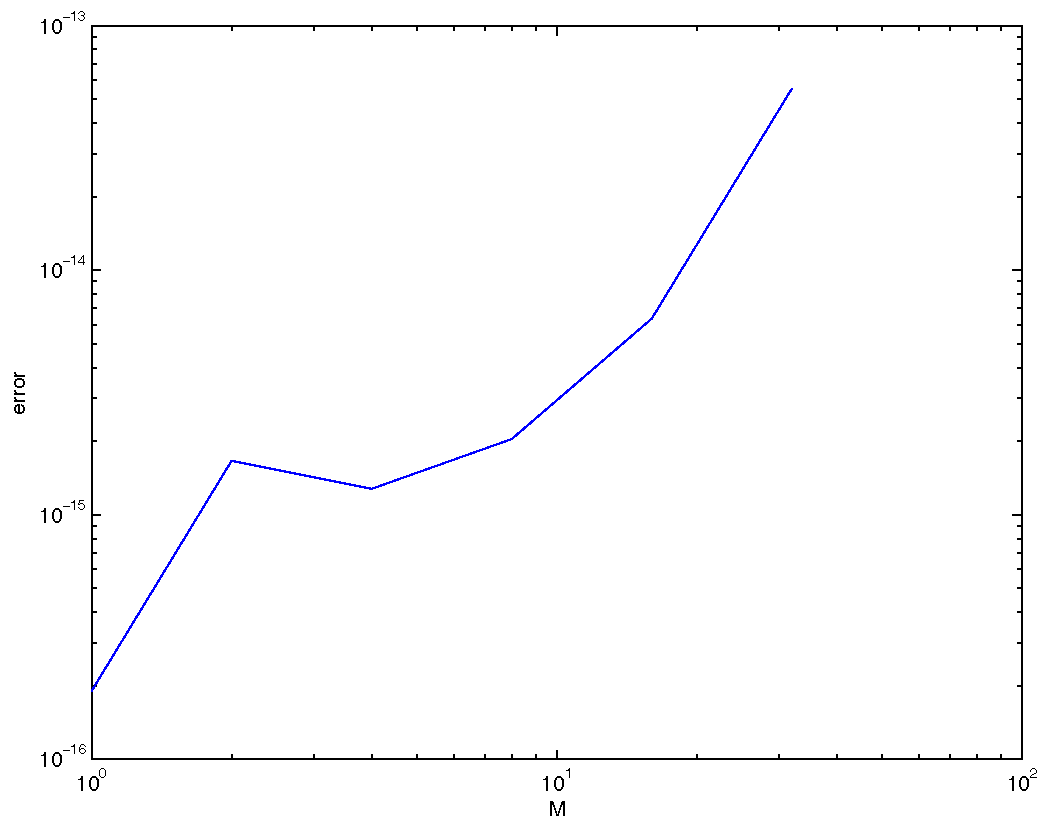
\includegraphics[height=9cm,width=12cm]{images/accuracy}
  \caption{To be written...}
  \label{NFSFT:Figure:Accuracy}
\end{figure}

This holds only in the case of equispaced nodes. If one leaves 
In this chapter, we first derive an algorithm for the fast evaluation of a bandlimited function $f$ at arbitrary nodes. Due to the separability 
of the basis functions $Y_k^n$, evaluating the sum in \eqref{NFSFT:FourierExpansion} can be split up in ordinary discrete Fourier transforms for nonequispaced 
data in colatitudinal direction and \emph{discrete Legendre function transforms} for the latitudinal part. The basic idea of the approach 
presented here is to perform a change of basis from Legendre functions to complex exponentials in latitudinal direction to get the 
representation
$$ \fun{f}{\vtheta,\vphi} = \sum_{n=-M}^{M} \sum_{k=-M}^M c_k^n e^{ik\vtheta} e^{in\vphi}.$$
The computation of the function values $f_j := \fun{f}{\vtheta_j,\vphi_j}$ can now be performed 
using a two-dimensional NFFT. 

Once derived a fast algorithm for this product, which implies a factorization of $\V{Y}$ into a product of sparse matrices,
one also immediately gets from the theoretical point of view a fast algorithm for the adjoint product 
$$\V{a} = \V{Y}^{\h} \; \V{f}.$$

\section{Fast Legendre Function Transform}
\label{DSFT:FLFT}

Let $M \in \NZ$ and $n \in \Z$ with $M \ge \abs{n}$ be given. The \index{Fast Legendre function transform} \emph{fast Legendre function transform (FLFT)}
considers polynomials of the form
$$ \fun{g_n}{x} := \sum_{k=\abs{n}}^M a_k^n \fun{P_k^{\abs{n}}}{x} \in \Pol_M$$
for even $n$ and
$$ \fun{g_n}{x} := \frac{1}{\sqrt{1-x^2}} \sum_{k=\abs{n}}^M a_k^n \fun{P_k^{\abs{n}}}{x} \in \Pol_M-1$$
for odd $n$ with given complex coefficients $a_k^n$. The FLFT computes the coefficients $b_k^n$ of the Chebyshev representation
$$ \fun{g_n}{x} = \sum_{k=0}^M b_k^n \fun{T_k}{x}$$
for even $n$ and
$$\fun{g_n}{x} = \sum_{k=0}^{M-1} b_k^n \fun{T_k}{x}$$
for odd $n$.

Lemma \ref{Basics:AssociatedLegendreRecurrence} implies
$$ 
  \left(\begin{array}{c}
    P_{c+k}^n \\ P_{c+k+1}^n
  \end{array}\right)
  =
  \fun{U_{k}^{n}}{\cdot,c}^{\transp}\;
  \left(\begin{array}{c}
    P_{c-1}^n \\ P_{c}^n
  \end{array}\right)
$$
where
$$
  \fun{U_{k}^{n}}{\cdot,c}^{\transp} :=
  \left(\begin{array}{cc}
    \gamma_c^n \fun{P_{k-1}^n}{\cdot,c+1} & \gamma_c^n \fun{P_{k}^n}{\cdot,c+1} \\
                             \fun{P_{k}^n}{\cdot,c}         &                         \fun{P_{k+1}^n}{\cdot,c}
  \end{array}\right).   
$$

We restrict ourselves to the case where $n$ is even. All further calculations will be performed with respect to $N$ as the 
bandwidth by setting $a_k^n := 0$ for $k < \abs{n}$ or $k > M$. In a first step, we use Lemma 
\ref{Basics:AssociatedLegendreRecurrence} to write
$$ g_n = \sum_{k = \abs{n}}^{N-1} a_{k}^{(0)} P_k^{\abs{n}} = \sum_{l = 0}^{\frac{N}{4}-1} \paren{\sum_{k = 0}^3 a_{4l+k}^{(0)}P_{4l+k}^{\abs{n}}},$$
with
\begin{eqnarray*}
  \fun{a_k^{(0)}}{x}     & := & a_k^n \quad (k = 0,\ldots,N-3),\\
  \fun{a_{N-2}^{(0)}}{x} & := & a_{N-2}^n + \gamma_{N-1}^{\abs{n}} a_N^n,\\
  \fun{a_{N-1}^{(0)}}{x} & := & a_{N-1}^n + \paren{\alpha_{N-1}^{\abs{n}}x + \beta_{N-1}^{\abs{n}}} a_N^n.
\end{eqnarray*}
Please take note of the fact that $a_k^{(0)}$  instead of constants are now polynomials of 
maximal degree $1$ and that one immediately has their corresponding Chebyshev coefficients.

From \eqref{} with $k = 1$ and $c = l+1$ it follows that
$$
\left(\begin{array}{c}
  P_{4l+2}^{|n|}, 
  P_{4l+3}^{|n|}
\end{array}\right)
\left(\begin{array}{c}
  a_{4l+2}^{(0)}\\
  a_{4l+3}^{(0)} 
\end{array}\right)
=
\left(\begin{array}{c}
  P_{4l}^{|n|},
  P_{4l+1}^{|n|}
\end{array}\right)
{\mathbf{U}_{1}^{|n|}\left(\cdot,4l+1\right)}
\left(\begin{array}{c}
  a_{4l+2}^{(0)}\\
  a_{4l+3}^{(0)} 
\end{array}\right)
$$
for $l=0,\ldots,\frac{}{}$and therefore
$$ g_n = \sum_{l = 0}^{\frac{M}{4}-1} a_{4l}^{(1)} P_{4l}^{\abs{n}} + a_{4l+1}^{(1)} P_{4l+1}^{\abs{n}} $$
with
\begin{equation}
\label{NFSFT:FirstStep}
  \left(\begin{array}{c}
    a_{4l}^{(1)}\\
    a_{4l+1}^{(1)} 
  \end{array}\right)
  =
  \left(\begin{array}{c}
    a_{4l}^{(0)}\\
    a_{4l+1}^{(0)} 
  \end{array}\right)
  + {\mathbf{U}_{1}^{|n|}\left(\cdot,4l+1\right)}
  \left(\begin{array}{c}
    a_{4l+2}^{(0)}\\
    a_{4l+3}^{(0)} 
  \end{array}\right).
\end{equation}
We can use Algorithm \ref{Basics:Algorithm:FastPolynomialMultiplication} with $N=2$ to compute 
the polynomial products in \eqref{NFSFT:FirstStep}. Applying this idea repeatedly leads to a cascade 
summation as illustrated in Figure \ref{NFSFT:Figure:CascadeSummation} calculating in step $\tau$
\begin{equation}
  \nonumber
  \left(\begin{array}{c}
    a_{2^{\tau+1}l}^{(\tau)}\\
    a_{2^{\tau+1}l+1}^{(\tau)} 
  \end{array}\right)
  =
  \left(\begin{array}{c}
    a_{2^{\tau+1}l}^{(\tau-1)}\\
    a_{2^{\tau+1}l+1}^{(\tau-1)} 
  \end{array}\right)
  + {\mathbf{U}_{2^{\tau}-1}^{|n|}\left(\cdot,2^{\tau+1}l+1\right)}
  \left(\begin{array}{c}
    a_{2^{\tau+1}l+2}^{(\tau-1)}\\
    a_{2^{\tau+1}l+3}^{(\tau-1)} 
  \end{array}\right).
\end{equation}
by applying Algorithm \ref{Basics:Algorithm:FastPolynomialMultiplication} with $N=2^{\tau}$. 
After step $j-1$ we arrive at
\begin{equation}
  \nonumber
  g_n = a_{0}^{j-1} P_{0}^{\abs{n}} + a_{1}^{j-1} P_{1}^{\abs{n}}
\end{equation}
Since 
\begin{align}
  \nonumber
  P_{0}^n(x) & = \frac{\left( \left( 2n \right) ! \right)^{1/2}}{2^n n!}, & P_{1}^n(x) & = \left(\alpha_{0}^nx + \beta_{0}^n\right)P_{0}^n(x)
\end{align} 
we get
\begin{equation}
  \label{NFSFT:LastStep}
  g_n = \frac{\left( \left( 2n \right) ! \right)^{1/2}}{2^n n!} a_{0}^{j-1} + a_{1}^{j-1} \left(\alpha_{0}^nx + \beta_{0}^n\right)P_{0}^n(x)
\end{equation}
Using 
\begin{equation}
  \nonumber
  xT_{0}(x) = T_{1}(x),\ xT_{k}(x) = \frac{1}{2}\left( T_{k+1}(x) + T_{k-1}(x) \right)
\end{equation}
one can calculate the remaining polynomial products in \eqref{NFSFT:LastStep} with elementary 
vector operations to yield the Chebyshev coefficients of $g_n$. The case, where $n$ is odd can 
be treated similarly and differs mainly in the last step.

\begin{figure}
  \label{NFSFT:Figure:CascadeSummation}
  % Cascade summation
  \unitlength0.87cm
    \begin{picture}(14,14)
      % setze 6 Boxen
      \multiput(0,0)(0,2.5){6}{\framebox(14,1)[lb]}
      % schreibe in die 1. Box
      \multiput(1.64,12.5)(1.64,0){8}{\line(0,1){1}}
      %\put(14.4,12.8){\large $\in \mathbb R$}
      \put(0.3,12.8){\large $0$}
      \put(1.0,12.8){\large $0$}
      \put(1.94,12.8){\large $0$}
      \put(2.64,12.8){\large $0$}
      \put(3.59,12.8){\large $a_4^4$}
      \put(4.29,12.8){\large $a_5^4$}
      \put(5.24,12.8){\large $a_6^4$}
      \put(5.94,12.8){\large $a_7^4$}
      \put(6.88,12.8){\large $a_8^4$}
      \put(7.58,12.8){\large $a_9^4$}
      \put(8.45,12.8){\large $a_{10}^4$}
      \put(9.15,12.8){\large $a_{11}^4$}
      \put(10.1,12.8){\large $a_{12}^4$}
      \put(10.8,12.8){\large $a_{13}^4$}
      \put(11.75,12.8){\large $a_{14}^4$}
      \put(12.4,12.8){\large $a_{15}^4$}
      \put(13.3,12.8){\large $a_{16}^4$}
      % schreibe zwischen 2. und 3. Box
      \multiput(12.2,11.5)(1.3,0){2}{\line(0,1){1}}
      \put(12.2,11.5){\line(1,0){1.3}}
      \put(12.7,11){\line(0,1){0.5}}
      %\multiput(0.82,11)(1.64,0){7}{\line(0,1){1.5}}
      \multiput(4.12,11)(1.64,0){5}{\line(0,1){1.5}}
      % schreibe in die 2. Box
      \multiput(1.64,10)(1.64,0){7}{\line(0,1){1}}
      %\put(14.4,10.3){\large $\in \Pi_1$}
      \put(0.2,10.3){\large $0$}
      \put(0.9,10.3){\large $0$}
      \put(1.8,10.3){\large $0$}
      \put(2.5,10.3){\large $0$}
      \put(3.5,10.3){\large $a_4^{(0)}$}
      \put(4.2,10.3){\large $a_5^{(0)}$}
      \put(5.1,10.3){\large $a_6^{(0)}$}
      \put(5.8,10.3){\large $a_7^{(0)}$}
      \put(6.75,10.3){\large $a_8^{(0)}$}
      \put(7.45,10.3){\large $a_9^{(0)}$}
      \put(8.35,10.3){\large $a_{10}^{(0)}$}
      \put(9.05,10.3){\large $a_{11}^{(0)}$}
      \put(10.05,10.3){\large $a_{12}^{(0)}$}
      \put(10.7,10.3){\large $a_{13}^{(0)}$}
      \put(12.05,10.3){\large $a_{14}^{(0)}$}
      \put(13.1,10.3){\large $a_{15}^{(0)}$}
      % schreibe zwischen 2. und 3. Box
      %\multiput(0.82,9)(1.64,0){7}{\line(0,1){1}}
      \multiput(4.10,9)(1.64,0){5}{\line(0,1){1}}
      \put(12.8,9){\line(0,1){1}}
      %\multiput(0.82,9)(3.28,0){3}{\line(1,0){1.64}}
      \multiput(4.10,9)(3.28,0){2}{\line(1,0){1.64}}
      \put(10.66,9){\line(1,0){2.14}}
      %\multiput(1.64,8.5)(3.28,0){4}{\line(0,1){0.5}}
      \multiput(4.92,8.5)(3.28,0){3}{\line(0,1){0.5}}
      %\put(0.95,9.3){$ U_1^4(\, \cdot\, ,1)$}
      \put(4.23,9.3){$ U_1^4(\, \cdot\, ,5)$}
      \put(7.45,9.3){$ U_1^4(\, \cdot\, ,9)$}
      \put(10.79,9.3){$ U_1^4(\; \cdot\; ,13)$}
      % schreibe in die 3. Box
      \multiput(3.3,7.5)(3.3,0){3}{\line(0,1){1}}
      %\put(14.4,7.8){\large $\in \Pi_3$}
      \put(0.82,7.8){\large $0$}
      \put(2.2,7.8){\large $0$}
      \put(3.8,7.8){\large $a_4^{(1)}$}
      \put(5.5,7.8){\large $a_5^{(1)}$}
      \put(7,7.8){\large $a_8^{(1)}$}
      \put(8.8,7.8){\large $a_9^{(1)}$}
      \put(10.5,7.8){\large $a_{12}^{(1)}$}
      \put(12.5,7.8){\large $a_{13}^{(1)}$}
      % schreibe zwischen 3. und 4. Box
      \multiput(1.64,6.5)(3.28,0){4}{\line(0,1){1}}
      \put(1.64,6.5){\line(1,0){3.28}}
      \put(8.2,6.5){\line(1,0){3.28}}
      \multiput(3.3,6.0)(6.6,0){2}{\line(0,1){0.5}}
      \put(2.4,6.8){$ U_3^4(\; \cdot\; ,1)$}
      \put(9.2,6.8){$ U_3^4(\; \cdot\; ,9)$}
      % schreibe in die 4. Box
      %\put(14.4,5.5){\large $\in \Pi_7$}
      \put(6.5,5){\line(0,1){1}}
      \put(2,5.3){\large $a_0^{(2)}$}
      \put(4,5.3){\large $a_1^{(2)}$}
      \put(8.5,5.3){\large $a_8^{(2)}$}
      \put(10.5,5.3){\large $a_9^{(2)}$}
      % schreibe zwischen 4. und 5. Box
      \multiput(3.3,4.0)(6.6,0){2}{\line(0,1){1}}
      \put(3.3,4){\line(1,0){6.6}}
      \put(5.8,4.3){$ U_7^4(\; \cdot\; ,1)$}
      \put(6.5,3.5){\line(0,1){0.5}}
      \put(6.5,1){\line(0,1){1.5}}
      % schreibe in die 4. Box
      %\put(14.4,2.8){\large $\in \Pi_{15}$}
      %\put(14.4,0.3){\large $\in \Pi_{16}$}
      \put(3,2.8){\large $a_0^{(3)}$}
      \put(9.5,2.8){\large $a_1^{(3)}$}
      \put(6.2,0.3){\large $\left(g_4(\cos\frac{s\pi}{16})\right)_{s=0,\ldots,16}$}
    \end{picture}
  \caption{To be written...}
\end{figure}

\begin{algorithm}[ht]
  \caption{Fast Legendre Function transform}
  \label{NFSFT:Algorithm:FLFT}    
  \begin{algorithmic}
    \STATE Input:  $M \in \NZ$, $n \in \Z$ $(\abs{n} \le M)$, $\paren{a_k^n}_{k=\abs{n},\ldots,M}$
    \STATE Precompute: $j := \ceil{\log_2 M}$, $N := 2^j$, $\fun{U_{2^{\tau}-1}^{\abs{n}}}{\cos \frac{\paren{2s+1}\pi}{2^{\tau+2}}, 2^{\tau+1}l+1}$ 
    \STATE \invisible{Precompute:} for $\tau 1,\ldots,j-1$, $l = \floor{\frac{\abs{n}}{2^{\tau+1}}},\ldots,\ceil{\frac{M}{2^{\tau+1}}}-1$ and
    \STATE \invisible{Precompute:} 

    \FOR {$j=0,\ldots , 2N-1$} 
      \STATE $f_{j} := \fun{P}{\cos \frac{(2j+1)\pi}{4N}} \fun{Q}{\cos \frac{(2j+1)\pi}{4N}}$
    \ENDFOR
    \STATE Output: $\paren{c_{k}}_{k=0}^{2N-1}$
\end{algorithmic}
\end{algorithm}


\section{Stabilization}
\label{DSFT:Stabilization}

\section{Nonuniform Fast Spherical Fourier Transform}
\label{DSFT:NFSFT}

\section{A Linear Algebra Approach}
\label{DSFT:LinearAlgebra}

In this section we represent the FLFT algorithm as a linear operator, hence a matrix, that acts on a vector of Fourier-coefficients. So let $M \in \N$ be a fixed bandwidth and as usual $t := \lceil\log_2{M}\rceil$, $N := 2^t$. Furthermore let  $-M \le n \le M$ be fixed. The FLFT can be represented as a matrix $\mb{T} \in \R^{(N+1) \times (N+1)}$ that multiplied with a vector $\mb{a} = \left(a_0^n,a_1^n,\dots,a_N^n\right)^T \in \C^{N+1}$ of Fourier coefficients gives a vector $\mb{g}_n = \left(g_0^n,g_1^n,\dots,g_{2N-1}^n\right) \in \C^{2N}$ containing the Chebyshev coefficients of the polynomial $g_n$: $$\mb{g_{n}} = \mb{T} \; \mb{a}.$$ For the sake of simplicity we omit the fact that $a_{k}^n = 0$ for $k < n$ or $k > M$. Clearly, this can be exploited in the algorithm to save some computational steps.

Since the FLFT algorithm is asymptotically faster than the naive evaluation of the polynomial $g_{n}$ at the Chebyshev nodes, this implies a factorization of $\mb{T}$ into sparse matrices. This factorization can be derived directly from the algorithm already presented and will later be used to construct an algorithm for the transposed problem. In general the FLFT consists of $t+1$ steps so that $\mb{T}$ can be written as $$\mb{T} = \mb{T}_{t} \: \cdot \:  \mb{T}_{t-1} \dots \mb{T}_{1} \: \cdot \:  \mb{T}_{0} \text{, with } \mb{T}_{\tau} \in \left\{\begin{array}{l@{\quad \text{if} \quad}l} \R^{2N \times (N+1)} & \tau = 0, \\ \R^{2N \times 2N} & 1 \le \tau < t, \\ \R^{(N+1) \times 2N} & \tau = t. \end{array}\right.$$

\subsubsection{The First Step}

The first step consists in converting each Fourier-coefficent $a_{k}^n$ into a polynomial of degree at most 1 in Chebyshev representation $\mb{a}_{k}^{(0)} \in \C^2$ so that the result $\mb{a^{(0)}}$ is a vector of length $2N$, hence $$ \mb{a}_{k}^{(0)} = \mb{e}_{1} a_{k}^n,\quad \text{with } \mb{e}_{1} = \left(\begin{array}{l}1\\0\end{array}\right).$$
The last polynomial $\mb{a}_{N}^{(0)}$ is mapped to the preceeding two polynomials by means of the three term recurrence for associated Legendre Functions, i.e. $\mb{a}_{N}^{(0)} = \left(\alpha x + \beta\right)\mb{a}_{N-1}^{(0)} + \gamma \mb{a}_{N-2}^{(0)}$. Following this, $\mb{T}_{0}$ can be written as
$$\left(\mb{I}_{N} \otimes \mb{e}_{1},\;\mb{\tilde{e}}\right),$$ 
where $\mb{\tilde{e}} = \left(0,0,\dots,0,\gamma, 0, \beta,\alpha\right)^T \in \R^{2N}.$

\subsubsection{Cascade Summation}

Steps $1$ to $t-1$ represent the cascade summation that is applied to associated Legendre functions. In each round, half of the the functions is eliminated by mapping them to the remaining functions. Therefore the vector is divided into consecutive blocks, each consisting of four polynomials representing the factors in front of each function. Each polynomial is represented by its vector of Chebyshev coefficients of length $2^{\tau}$. In every block, the first and the second polynomial remain unchanged. The third and the fourth polynomial are multiplied with a matrix $\mb{U}$ that transforms them into a representation in terms of the first two functions. Following this, the output contains only half of the polynomials compared to the input vector, but due to the multiplication with $\mb{U}$ the degree might double each time so that twice the space is needed to store the Chebyshev coefficients. So in total the result vector still has length $2N$. For each step $1 \le \tau < t$ and for each block $$\mb{\tilde{a}}_{l}^{(\tau-1)} := \left(\mb{a}_{4l}^{(\tau-1)},\mb{a}_{4l+1}^{(\tau-1)},\mb{a}_{4l+2}^{(\tau-1)},\mb{a}_{4l+3}^{(\tau-1)}\right)^T \text{, where } 0 \le l < 2^{t-\tau-1},$$ we need to keep the first two polynomials but with their vectors zero-padded up to twice the length. Furthermore, the multiplication with the matrix $\mb{U}$ acts on the third and fourth polynomial.
Correspondingly, each block $\mb{\tilde{a}}_{l}^{(\tau-1)}$ is multiplied by a matrix $\mb{V}_{\tau}^l := \left[\mb{Z_{\tau}},\mb{U}_{\tau}^l\right]$, with
$$\mb{Z}_{\tau} := \left(\begin{array}{cccc} \mb{I}_{2^{\tau}} & 0\\ 0 & 0 \\ 0 & \mb{I}_{2^{\tau}} \\ 0 & 0 \end{array}\right) \in \R^{2^{\tau+2} \times 2^{\tau+1}},\ \mb{U}_{\tau}^l \in \R^{2^{\tau+2} \times 2^{\tau+1}}.$$
%Correspondingly, this can be written as the product 
%$$\mb{ZP}_{\tau} \; \mb{\tilde{a}}_{l}^{\tau-1} \text{, with } \mb{ZP}_{\tau} := \left(\begin{array}{cccc} \mb{I}_{2^{\tau}} & 0 & 0 & 0\\ 0 & 0 & 0 & 0 \\ 0 & \mb{I}_{2^{\tau}} & 0 & 0 \\ 0 & 0 & 0 & 0 \end{array}\right) \in \R^{2^{\tau+2} \times 2^{\tau+2}}.$$ 
%The multiplication with the matrix $\mb{U}$ that acts on the third and fourth polynomial is written as $\mb{U}_{\tau}^l \; \mb{\tilde{a}}_{l}^{\tau-1}$ where the matrix can be factorized as follows:
The matrix $\mb{U}_{\tau}^l$ can be factorized as follows:
$$ \mb{U}_{\tau}^l = \mb{D}_{\tau}^{II} \; \cdot \; \mb{S}_{\tau} \; \cdot \; \mb{P}_{\tau}\left(2^{\tau + 1}l+1\right) \; \cdot \; \mb{D}_{\tau}^{III}  \in \R^{2^{\tau+2} \times 2^{\tau+1}}$$
where we define
\begin{eqnarray*}
  \mb{D}_{\tau}^{II} & := & \mb{I}_{2} \otimes \left(\mb{\tilde{D}}_{2^{\tau+1}} \mb{\tilde{C}}_{2^{\tau+1}}\right) \in \R^{2^{\tau+2} \times 2^{\tau+2}},\\
  \mb{S}_{\tau} & := & \mb{I}_2 \otimes \left[\begin{array}{cc}\mb{I}_{2^{\tau+1}},\mb{I}_{2^{\tau+1}}\end{array}\right] \in \R^{2^{\tau+2} \times 2^{\tau+3}},\\
  \mb{P}_{\tau}(c) & := & \text{diag}\left(\gamma_{c}^n \mb{P}_{2^{\tau}-2}^n(c+1),\gamma_{c}^n \mb{P}_{2^{\tau}-1}^n(c+1),\right.\\
    & & \left. \mb{P}_{2^{\tau}-1}^n(c), \mb{P}_{2^{\tau}}^n(c)\right) \in \R^{2^{\tau+3} \times 2^{\tau+3}},\\
  \mb{D}_{\tau}^{III} & := &\mb{I}_{2} \otimes \left(\left(\mb{I}_{2} \otimes \mb{\tilde{C}}^T_{2^{\tau+1}}\right)\mb{Z}_{\tau}\right) \in \R^{2^{\tau+3} \times 2^{\tau+1}}.
\end{eqnarray*}   
This interpretation corresponds directly to the algorithm implemented. The matrix $\mb{D}_{\tau}^{III}$ realizes first the zero-padding of the two polynomials ($\mb{Z}$), second the evaluation of the polynomials at the Chebyshev nodes ($\mb{\tilde{C}}^T$) and finally a duplication of the result vector in order to permit multiplication with two different associated Legendre functions for each polynomial. The matrix $\mb{P}_{\tau}(c)$ contains the associated Legendre polynomials of the matrix $U_{2^{\tau}-1}^n(\cdot,2^{\tau+1}l+1)$ also evaluated at the Chebyshev nodes on its main diagonal. Therefore a multiplication with this matrix realizes a pointwise multiplication of the zero-padded and evaluated polynomials. For each of the two rows of $U_{2^{\tau}-1}^n(\cdot,2^{\tau+1}l+1)$, two of the results of the previous step are summed by the following multiplication with the matrix $\mb{S}_{\tau}$. Finally, the matrix $\mb{D}_{\tau}^{II}$ transforms the newly formed polynomials back into Chebyshev coefficients.

From the factorization a more compact representation can be obtained, so that $\mb{U}_{\tau}^l$ can be written as
\begin{equation}
\label{UCompact}
\mb{U}_{\tau}^l = 
\left(\begin{array}{lclrcr}
\mb{\mb{\tilde{D}}_{2^{\tau+1}}\tilde{C}}_{2^{\tau+1}} & \gamma_{c}^n & \left(\right. & \mb{P}_{2^{\tau}-2}^n(c+1) \mb{\tilde{C}}^T_{2^{\tau+1}} Z_{1} & + & \mb{P}_{2^{\tau}-1}^n(c+1) \mb{\tilde{C}}^T_{2^{\tau+1}} Z_{2} \left.\right) \\
\mb{\mb{\tilde{D}}_{2^{\tau+1}}\tilde{C}}_{2^{\tau+1}} & & \left(\right. & \mb{P}_{2^{\tau}-1}^n(c) \mb{\tilde{C}}^T_{2^{\tau+1}} Z_{1} & + & \mb{P}_{2^{\tau}}^n(c) \mb{\tilde{C}}^T_{2^{\tau+1}} Z_{2} \left.\right)
\end{array}\right)
\end{equation}
%So for each block $l$, a multiplication with a matrix $\mb{V}_{\tau}^l  \in \R^{2^{\tau+2} \times 2^{\tau+2}}$ is applied where
%$$ \mb{V}_{\tau}^l = \left[\mb{ZP},\mb{U}_{\tau}^l\right].$$ 
The complete round can then be represented as $$\mb{T}_{\tau} = \text{diag}\left(\mb{V}_{\tau}^0,\mb{V}_{\tau}^1,\dots,\mb{V}_{\tau}^{2^{t-\tau-1}-1}\right).$$

\subsubsection{The Last Step}
The last step consists of calculating the polynomial $g_{n} = \mb{a}_{0}^{(t-1)} P_{0}^{|n|} + \mb{a}_{1}^{(t-1)} P_{1}^{|n|}$ in Chebyshev representation. Since 
$$P_{0}^n(x) = \frac{\left( \left( 2n \right) ! \right)^{1/2}}{2^n n!},\ P_{1}^n(x) = \left(\alpha_{0}^nx + \beta_{0}^n\right)P_{0}^n(x)$$ we can use 
$$xT_{0}(x) = T_{1}(x),\ xT_{k}(x) = \frac{1}{2}\left( T_{k+1}(x) + T_{k-1}(x) \right)$$ to write
$$ \mb{g_{n}} = \gamma_{0}^n \left( \mb{I}_{N+1} \mb{a}_{0}^{(\tau-1)} + \left( \alpha_{0}^n\mb{W}_{N+1} + \beta_{0}^n\mb{I}_{N+1} \right) \mb{a}_{1}^{(\tau-1)} \right)$$
Depending on $n \in \N_{0}$, we can distinguish three cases:
\begin{description}
  \item[n odd:] In this case, $\alpha_{0}^n = 0$ and $\beta_{0}^n = 1$ so that $\mb{T}_{\tau}$ can be written as $$\mb{T}_{\tau} = \gamma_{0}^n \left[ \mb{I}_{N+1}, \mb{I}_{N+1} \right].$$
  \item[n = 0:] Here it holds, $\alpha_{0}^n = 1$ and $\beta_{0}^n = 0$ and we get $$\mb{T}_{\tau} = \gamma_{0}^n \left[ \mb{I}_{N+1}, \mb{W}_{N+1} \right].$$
  \item[n even, n > 0:] Now $\alpha_{0}^n = -1$ and $\beta_{0}^n = 1$ which results in $$\mb{T}_{\tau} = \gamma_{0}^n \left[ \mb{I}_{N+1}, \mb{I}_{N+1} - \mb{W}_{N+1} \right].$$
\end{description}
where we define
$$
\mb{W}_{n} :=
\left(
\begin{array}{ccccccc}
  0 & \frac{1}{2} &             &                           \\
  1 &           0 & \frac{1}{2} &                           \\
    & \frac{1}{2} &           0 & \ddots                    \\
    &             &      \ddots & \ddots      & \frac{1}{2} \\
    &             &             & \frac{1}{2} &           0
\end{array}
\right)
\in \R^{n \times n}.
$$

\subsection{The Adjoint Operator}
Following the factorization of $\mb{T}$ given in the previous section, one obtains easily the adjoint operator which is paramount for an implementation of xxx: 
$$\mb{T}^H = \mb{T}_{0}^H \; \cdot \; \mb{T}_{1}^H \dots \mb{T}_{t-1}^H \; \cdot \; \mb{T}_{t}^H.$$ For $\tau = 0$ and $\tau = t$ we obtain immediatly
$$ \mb{T}_{0}^H = \left( \begin{array}{c} \mb{I}_{N} \otimes \mb{e}_{1}^T\\ \mb{\tilde{e}}^T \end{array}\right), \mb{T}_{t}^H = \gamma_{0}^n \left\{\begin{array}{l@{\quad \text{if} \quad}l} 
 \left[ \begin{array}{c} \mb{I}_{N+1} \\ \mb{I}_{N+1} \end{array} \right] & \text{n odd},\\[2ex]
 \left[ \begin{array}{c} \mb{I}_{N+1} \\ \mb{T}_{N+1}^T \end{array} \right] & \text{n = 0},\\[2ex]
 \left[ \begin{array}{c} \mb{I}_{N+1} \\ \mb{I}_{N+1} - \mb{T}_{N+1}^T \end{array} \right] & \text{n even, n > 0}.
\end{array}\right.$$
Using xxx we get for the rest of the steps $\mb{T}_{\tau}$, $1 \le \tau \le t-1$
\begin{eqnarray*}
 \mb{T}_{\tau}^H & = & \text{diag}\left({\mb{V}_{\tau}^0}^H,{\mb{V}_{\tau}^1}^H,\dots,{\mb{V}_{\tau}^{2^{t-\tau-1}-1}}^H\right),\\
 {\mb{V}_{\tau}^l}^H & = & \left[ \begin{array}{c} \mb{Z}^H \\ { \mb{U}_{\tau}^l}^H \end{array} \right],\\
 {\mb{U}_{\tau}^l}^H & = &
   \left(
     \begin{array}{rlllr}
        \gamma_{c}^n & \left(\right. Z_{1}^T \mb{\tilde{C}}_{2^{\tau+1}} \mb{P}_{2^{\tau}-2}^n(c+1)   & + & Z_{2}^T \mb{\tilde{C}}_{2^{\tau+1}} \mb{P}_{2^{\tau}-1}^n(c+1)
         & \left.\right) \mb{\tilde{C}}_{2^{\tau+1}}^T \\
        & \left(\right. Z_{1}^T \mb{\tilde{C}}_{2^{\tau+1}} \mb{P}_{2^{\tau}-1}^n(c) & + & Z_{2}^T \mb{\tilde{C}}_{2^{\tau+1}} \mb{P}_{2^{\tau}}^n(c) & \left.\right) \mb{\tilde{C}}_{2^{\tau+1}}^T
     \end{array}
   \right).
\end{eqnarray*}


\section{Adjoint Fast Spherical Fourier Transform}
\label{DSFT:AdjointTransform}